\chapter{模型评估与选择}

% ============ §7.1 引言 ============
\section{引言}

学习方法的\textbf{泛化性能（generalization performance）}涉及其在独立测试数据上的预测能力。在实践中，评估这一性能极为重要——它指导学习方法或模型的选择，并给出最终所选模型质量的度量。

本章描述并展示性能评估的关键方法，以及如何利用它们进行模型选择。我们从偏差、方差和模型复杂度之间的交互关系开始讨论。

\section{偏差、方差与模型复杂度}

\begin{figure}[htbp]
    \centering
    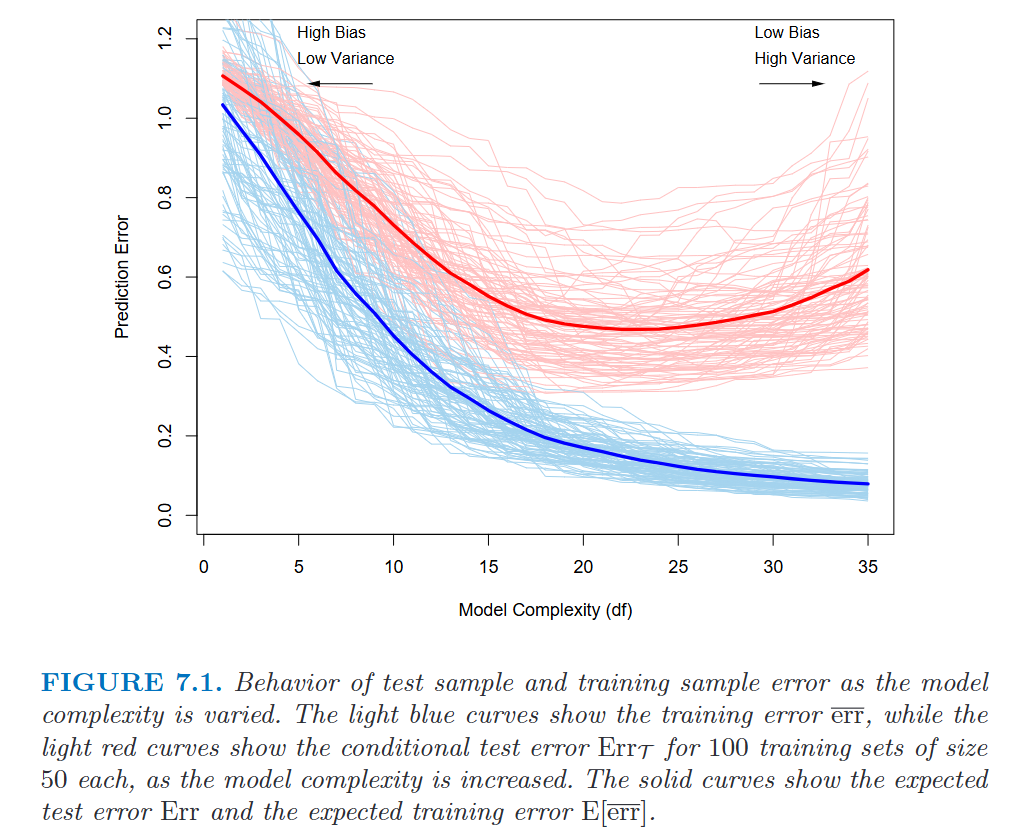
\includegraphics[width=0.95\textwidth]{Chapters/pic/ch_模型评估与选择/figure_7_1.png}
    \caption{测试误差和训练误差随模型复杂度变化的行为。浅蓝色曲线为训练误差 $\overline{\mathrm{err}}$，浅红色曲线为 100 个大小为 50 的训练集各自的条件测试误差 $\mathrm{Err}_{\mathcal{T}}$，随模型复杂度增加而变化。实线为期望测试误差 $\mathrm{Err}$ 和期望训练误差 $\E[\overline{\mathrm{err}}]$。}
    \label{fig:7_1}
\end{figure}

\subsection{定量响应情形}

对定量（区间尺度）响应 $Y$，给定输入向量 $X$ 和由训练集 $\mathcal{T}$ 估计的预测模型 $\hat{f}(X)$。损失函数 $L(Y, \hat{f}(X))$ 衡量预测误差，常见选择为：

\begin{itemize}
    \item \textbf{平方误差：} $L(Y, \hat{f}(X)) = (Y - \hat{f}(X))^2$
    \item \textbf{绝对误差：} $L(Y, \hat{f}(X)) = |Y - \hat{f}(X)|$
\end{itemize}

\textbf{测试误差（test error）}，也称泛化误差，是在独立测试样本上的预测误差：
\begin{equation}\label{eq:err_T}
    \mathrm{Err}_{\mathcal{T}} = \E_{X^0, Y^0}\bigl[L(Y^0, \hat{f}(X^0)) \mid \mathcal{T}\bigr]
\end{equation}
其中 $(X^0, Y^0)$ 是从联合分布（总体）中随机抽取的。训练集 $\mathcal{T}$ 固定，测试误差指该特定训练集的误差。

\subsubsection{$\mathrm{Err}_{\mathcal{T}}$ 中的 $(X^0, Y^0)$ 是从测试集中抽的吗？}

不是。$(X^0, Y^0)$ 并非从某个实际的「测试集」中抽取，而是从数据的\textbf{联合分布（总体）} $F$ 中随机抽取的。$\E_{X^0, Y^0}$ 是\textbf{对总体的积分}，而非对有限测试样本的平均。

区别在于：理论上 $\mathrm{Err}_{\mathcal{T}}$ 对所有可能的未来数据点取期望，衡量模型在\textbf{整个分布}上的表现；实践中我们只有一个有限的测试集，用其上的平均损失 $\frac{1}{M}\sum_{j=1}^{M} L(y_j^0, \hat{f}(x_j^0))$ 来\textbf{估计} $\mathrm{Err}_{\mathcal{T}}$。这就是 $\mathrm{Err}_{\mathcal{T}}$ 被称为「额外样本误差（extra-sample error）」的原因——测试输入向量不需要与训练输入向量重合。

与此相关的量是\textbf{期望预测误差（expected prediction error）}：
\begin{equation}\label{eq:Err}
    \mathrm{Err} = \E\bigl[L(Y^0, \hat{f}(X^0))\bigr] = \E[\mathrm{Err}_{\mathcal{T}}]
\end{equation}
该期望对一切随机因素取平均，包括产生 $\hat{f}$ 的训练集的随机性。

图7.1展示了100个大小为50的模拟训练集的预测误差曲线（浅红色），以及其平均（实红色，估计 $\mathrm{Err}$）。Lasso（第3.4.2节）用于产生拟合序列。

\subsubsection{如何区分不同训练集训练出的模型？}

$\hat{f}$ 依赖于训练集 $\mathcal{T}$，不同的 $\mathcal{T}$ 会拟合出不同的 $\hat{f}$。$\mathrm{Err}_{\mathcal{T}}$ 的下标 $\mathcal{T}$ 明确表示在\textbf{该特定训练集}上训练出的模型的测试误差。在图7.1中，100条浅红色曲线各对应一个不同的 $\mathcal{T}$，框架本身不需要额外的区分机制——$\mathcal{T}$ 的随机性已经刻画了这种差异。简言之：$\mathrm{Err}_{\mathcal{T}}$ 把 $\mathcal{T}$ 视为条件（固定），$\mathrm{Err}$ 把 $\mathcal{T}$ 视为随机变量（对其积分）。

\subsubsection{期望预测误差和测试误差的区别}

两个概念的区别在于\textbf{对什么取平均}：两者都对 $(X^0, Y^0)$ 在总体上积分，但 $\mathrm{Err}_{\mathcal{T}}$ 固定训练集 $\mathcal{T}$（是随机变量，取决于抽到哪份数据），而 $\mathrm{Err} = \E_{\mathcal{T}}[\mathrm{Err}_{\mathcal{T}}]$ 进一步对训练集取平均（是固定数，属于学习方法本身的属性）。

类比：$\mathrm{Err}_{\mathcal{T}}$ 像某个人的身高（取决于挑中谁），$\mathrm{Err}$ 像人群平均身高（固定参数）。ESL 更关注 $\mathrm{Err}$，因为它具有更好的统计可操作性——大多数方法（$C_p$、AIC、交叉验证等）实际估计的都是 $\mathrm{Err}$ 而非 $\mathrm{Err}_{\mathcal{T}}$。

\textbf{训练误差（training error）}是训练样本上的平均损失：
\begin{equation}\label{eq:err}
    \overline{\mathrm{err}} = \frac{1}{N}\sum_{i=1}^{N} L(y_i, \hat{f}(x_i))
\end{equation}

\subsubsection{$\overline{\mathrm{err}}$、$\mathrm{Err}_{\mathcal{T}}$、$\mathrm{Err}$ 三者的关系}

三个量构成一条从「可算」到「不可算」的链条：
\begin{equation}\label{eq:err_chain}
    \overline{\mathrm{err}} \;\le\; \mathrm{Err}_{\mathcal{T}} \;\approx\; \mathrm{Err}
\end{equation}

\begin{itemize}
    \item $\mathrm{Err}$ 是最终目标——它回答「这个\textbf{学习方法}从总体中反复抽样训练，平均表现如何」，是方法本身的属性，不依赖于某一份运气好坏的训练集。
    \item $\mathrm{Err}_{\mathcal{T}}$ 是「用手里这份 $\mathcal{T}$ 训练出的那个模型」在全体未来数据上的期望误差。它仍是对总体积分，但训练集固定，故 $\mathrm{Err} = \E_{\mathcal{T}}[\mathrm{Err}_{\mathcal{T}}]$。实践中我们只有一份 $\mathcal{T}$，只能接触到 $\mathrm{Err}_{\mathcal{T}}$，但\textbf{算不出来}（需要对总体积分）。
    \item $\overline{\mathrm{err}}$ 是唯一能直接算的量，但它是 $\mathrm{Err}_{\mathcal{T}}$ 的系统性偏低估计——同一批数据既拟合又评估，模型会「记忆」训练数据。
\end{itemize}

本章所有方法（$C_p$、AIC、交叉验证、Bootstrap）本质上都是在 $\overline{\mathrm{err}}$ 上加一个\textbf{乐观性修正项} $\hat{\omega}$，使其逼近 $\mathrm{Err}$（或 $\mathrm{Err}_{\mathcal{T}}$）：
\begin{equation}\label{eq:err_hat}
    \widehat{\mathrm{Err}} = \overline{\mathrm{err}} + \hat{\omega}
\end{equation}

随着模型越来越复杂，它更好地利用训练数据并适应更复杂的底层结构，因此\textbf{偏差减小但方差增大}。存在某个中间模型复杂度使期望测试误差达到最小。

\begin{remark}
    训练误差不是测试误差的良好估计（如图7.1所示）。训练误差随模型复杂度单调递减，若模型足够复杂甚至可以降至零。然而，\textbf{训练误差为零的模型是对训练数据过拟合的}，通常泛化能力很差。
\end{remark}

\subsection{定性响应情形}

对于取 $\mathcal{G}$ 中 $K$ 个值之一的定性（分类）响应 $G$，通常对概率 $p_k(X) = \Pr(G = k \mid X)$ 建模，然后 $\hat{G}(X) = \argmax_k \hat{p}_k(X)$。常见损失函数为：

\begin{itemize}
    \item \textbf{0-1损失：} $L(G, \hat{G}(X)) = I(G \neq \hat{G}(X))$
    \item \textbf{偏差（deviance）：}
    \begin{equation}\label{eq:deviance}
        L(G, \hat{p}(X)) = -2\sum_{k=1}^{K} I(G = k)\log \hat{p}_k(X) = -2\log \hat{p}_G(X)
    \end{equation}
    量 $-2 \times$ 对数似然也称为\textbf{偏差}。
\end{itemize}

测试误差 $\mathrm{Err}_{\mathcal{T}}$ 是分类器在总体上的误分类误差，$\mathrm{Err}$ 是期望误分类误差。训练误差为样本类似量，例如：
\begin{equation}
    \overline{\mathrm{err}} = -\frac{2}{N}\sum_{i=1}^{N} \log \hat{p}_{g_i}(x_i)
\end{equation}
即模型的样本对数似然。

\begin{remark}
    「$-2$」使得高斯分布下的对数似然损失与平方误差损失一致。为叙述方便，本章后续以定量响应（平方误差损失）为主，其他情形的适当变换是显然的。
\end{remark}

\subsection{模型选择 vs 模型评估}

本章的方法通常涉及调节参数 $\alpha$，预测记为 $\hat{f}_\alpha(x)$。调节参数改变模型复杂度，我们希望找到使误差最小的 $\alpha$。

需要区分两个目标：

\begin{itemize}
    \item \textbf{模型选择（Model selection）：} 估计不同模型的性能以选择最佳模型。
    \item \textbf{模型评估（Model assessment）：} 选定最终模型后，估计其在新数据上的预测误差（泛化误差）。
\end{itemize}

在数据充足的情况下，最佳做法是随机将数据分为三部分：

\begin{itemize}
    \item \textbf{训练集（training set）：} 用于拟合模型；
    \item \textbf{验证集（validation set）：} 用于估计预测误差以进行模型选择；
    \item \textbf{测试集（test set）：} 用于评估最终所选模型的泛化误差。
\end{itemize}

\begin{remark}
    理想情况下，测试集应被「锁在保险柜里」，仅在数据分析的最后阶段取出。若反复使用测试集——选择测试集误差最小的模型——则最终所选模型的测试集误差将\textbf{低估}真实测试误差，有时低得相当严重。
\end{remark}

本章的方法通过\textbf{解析近似}（AIC、BIC、MDL、SRM）或\textbf{高效的样本重复利用}（交叉验证和自助法）来近似验证步骤。

% ============ §7.3 偏差-方差分解 ============
\section{偏差-方差分解}

与第2章一样，假设 $Y = f(X) + \varepsilon$，其中 $\E(\varepsilon) = 0$，$\Var(\varepsilon) = \sigma_\varepsilon^2$。对回归拟合 $\hat{f}(X)$ 在输入点 $X = x_0$ 处的期望预测误差（使用平方误差损失），有如下分解：
\begin{equation}\label{eq:bias_var}
    \begin{aligned}
        \mathrm{Err}(x_0) &= \E\bigl[(Y - \hat{f}(x_0))^2 \mid X = x_0\bigr] \\
        &= \sigma_\varepsilon^2 + \bigl[\E\hat{f}(x_0) - f(x_0)\bigr]^2 + \E\bigl[\hat{f}(x_0) - \E\hat{f}(x_0)\bigr]^2 \\
        &= \sigma_\varepsilon^2 + \mathrm{Bias}^2(\hat{f}(x_0)) + \Var(\hat{f}(x_0)) \\
        &= \text{不可约误差} + \text{偏差}^2 + \text{方差}.
    \end{aligned}
\end{equation}

第一项是目标值围绕其真实均值 $f(x_0)$ 的方差，无论 $\hat{f}$ 多好都无法避免（除非 $\sigma_\varepsilon^2 = 0$）。第二项是\textbf{平方偏差}——估计的均值与真实均值之差；第三项是\textbf{方差}——估计围绕其均值的期望平方偏差。

\begin{remark}
    通常模型越复杂，平方偏差越低但方差越高。
\end{remark}

\subsection{$k$-最近邻回归的偏差-方差分解}

对 $k$-最近邻回归拟合，假设训练输入 $x_i$ 固定，随机性仅来自 $y_i$：
\begin{equation}\label{eq:knn_bias_var}
    \mathrm{Err}(x_0) = \E\bigl[(Y - \hat{f}_k(x_0))^2 \mid X = x_0\bigr]
    = \sigma_\varepsilon^2 + \left[f(x_0) - \frac{1}{k}\sum_{\ell=1}^{k} f(x_{(\ell)})\right]^2 + \frac{\sigma_\varepsilon^2}{k}
\end{equation}
邻居数 $k$ 与模型复杂度成反比。$k$ 小 → 能更好地适应 $f(x_0)$；$k$ 增大 → 偏差通常增大而方差减小。

\subsection{线性回归的偏差-方差分解}

对线性模型 $\hat{f}_p(x_0) = x_0^T \hat{\beta}$ 使用最小二乘拟合：
\begin{equation}\label{eq:linear_bias_var}
    \mathrm{Err}(x_0) = \sigma_\varepsilon^2 + \bigl[f(x_0) - \E\hat{f}_p(x_0)\bigr]^2 + \norm{h(x_0)}^2 \sigma_\varepsilon^2
\end{equation}
其中 $h(x_0) = X(X^T X)^{-1} x_0$，是产生拟合的 $N$ 维线性权重向量。该方差虽随 $x_0$ 变化，但其平均值（以样本值 $x_i$ 为 $x_0$）为 $(p/N)\sigma_\varepsilon^2$，从而得到样本内误差：
\begin{equation}\label{eq:in_sample_err_linear}
    \frac{1}{N}\sum_{i=1}^{N} \mathrm{Err}(x_i) = \sigma_\varepsilon^2 + \frac{1}{N}\sum_{i=1}^{N}\bigl[f(x_i) - \E\hat{f}_p(x_i)\bigr]^2 + \frac{p}{N}\sigma_\varepsilon^2
\end{equation}
复杂度直接与参数个数 $p$ 相关。

\subsection{岭回归的偏差分解}

对岭回归拟合 $\hat{f}_\alpha(x_0)$，检验误差形式与 \eqref{eq:linear_bias_var} 相同，但方差项中的线性权重不同：$h(x_0) = X(X^T X + \alpha I)^{-1} x_0$。偏差项也不同。

对线性模型族（如岭回归），偏差可进一步精细分解。设 $\beta_*$ 为 $f$ 的最佳线性逼近参数：
\begin{equation}
    \beta_* = \argmin_\beta \E\bigl[f(X) - X^T\beta\bigr]^2
\end{equation}
期望关于输入变量 $X$ 的分布。则平均平方偏差可写为：
\begin{equation}\label{eq:bias_decomp}
    \begin{aligned}
        \E_{x_0}\bigl[f(x_0) - \E\hat{f}_\alpha(x_0)\bigr]^2
        &= \E_{x_0}\bigl[f(x_0) - x_0^T\beta_*\bigr]^2
           + \E_{x_0}\bigl[x_0^T\beta_* - \E(x_0^T\hat{\beta}_\alpha)\bigr]^2 \\
        &= \text{Ave[模型偏差]} + \text{Ave[估计偏差]}
    \end{aligned}
\end{equation}

\begin{itemize}
    \item \textbf{模型偏差（Model Bias）：} 最佳线性逼近与真实函数之间的误差——只能通过将线性模型族扩大为更丰富的模型集合（如引入交互项和变量变换）来减小。
    \item \textbf{估计偏差（Estimation Bias）：} 平均估计与最佳线性逼近之间的误差。OLS的估计偏差为零；受限拟合（如岭回归）的估计偏差为正，我们用它换取方差的降低。
\end{itemize}

\begin{figure}[htbp]
    \centering
    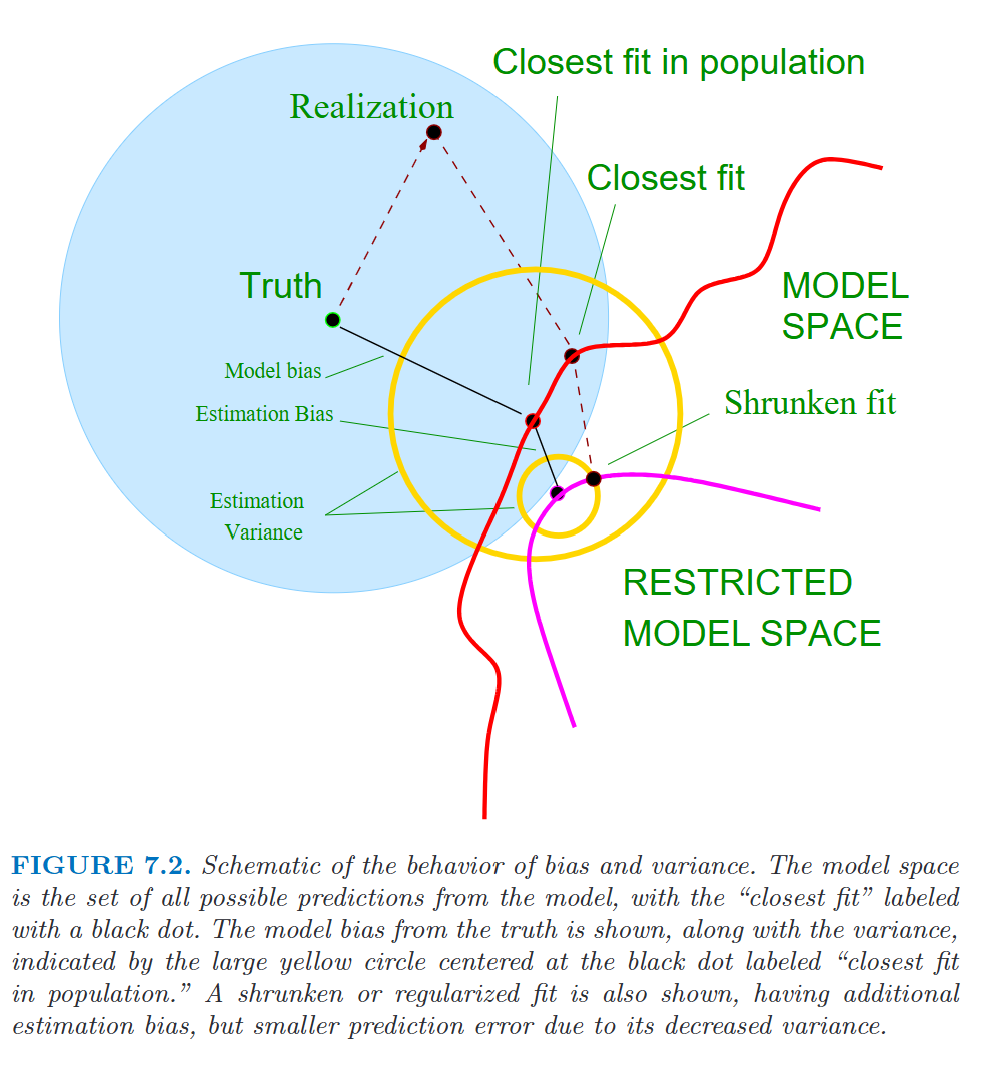
\includegraphics[width=0.85\textwidth]{Chapters/pic/ch_模型评估与选择/figure_7_2.png}
    \caption{偏差与方差行为的示意图。模型空间是模型所有可能预测的集合，「最近拟合」以黑点标出。真值与最近拟合之间的距离为模型偏差。方差由以「总体中的最近拟合」为中心的大黄色圆表示。收缩/正则化拟合具有额外的估计偏差，但由于方差减小，预测误差反而更小。}
    \label{fig:7_2}
\end{figure}

若用更少的预测变量或对系数向零收缩来拟合模型，则得到「收缩拟合」。该拟合离模型空间中的最佳拟合更远（增加了估计偏差），但方差更小。若方差减少超过（平方）偏差的增加，则这种收缩是值得的。

\subsection{示例：偏差-方差权衡}

\begin{figure}[htbp]
    \centering
    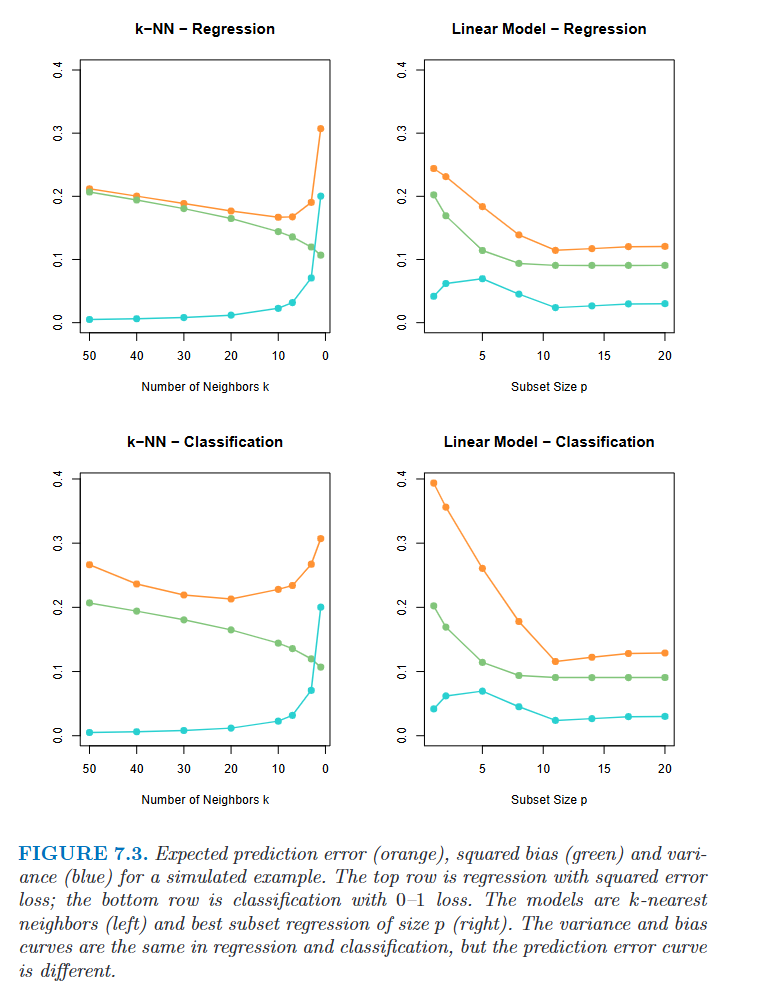
\includegraphics[width=0.95\textwidth]{Chapters/pic/ch_模型评估与选择/figure_7_3.png}
    \caption{模拟示例的期望预测误差（橙色）、平方偏差（绿色）和方差（蓝色）。上行：平方误差损失的回归；下行：0-1损失的分类。左列：$k$-最近邻；右列：大小为 $p$ 的最佳子集线性回归。偏差和方差曲线在回归与分类中相同，但预测误差曲线不同。}
    \label{fig:7_3}
\end{figure}

共有80个观测和20个预测变量，均匀分布在超立方体 $[0,1]^{20}$ 中：

\begin{itemize}
    \item \textbf{左侧面板：} $Y$ 当 $X_1 \le 1/2$ 时为0，否则为1，使用 $k$-最近邻。
    \item \textbf{右侧面板：} $Y$ 当 $\sum_{j=1}^{10} X_j > 5$ 时为1，否则为0，使用大小为 $p$ 的最佳子集线性回归。
\end{itemize}

上行是平方误差损失的回归；下行是0-1损失的分类。图中展示了预测误差（红色）、平方偏差（绿色）和方差（蓝色），均在大型测试样本上计算。

\textbf{回归情形：}偏差和方差相加产生预测误差曲线，最小值出现在 $k \approx 5$（$k$-NN）和 $p \ge 10$（线性模型）。

\textbf{分类情形（下行）：}出现了一些有趣现象：
\begin{itemize}
    \item 偏差和方差曲线与上行相同，但预测误差现在指误分类率。
    \item 预测误差\textbf{不再是平方偏差与方差之和}。
    \item 对 $k$-NN分类器，当邻居数从1增加到20时，预测误差下降或保持不变，尽管平方偏差在上升。
    \item 对线性模型分类器，最小值和回归一样在 $p \ge 10$ 处，但相比 $p=1$ 的改进更为显著。
    \item 偏差和方差似乎在决定预测误差时存在\textbf{交互作用}。
\end{itemize}

% ============ §7.4 训练误差的乐观性 ============
\section{训练误差的乐观性}

关于误差率估计的讨论可能令人困惑，因为需要明确哪些量是固定的、哪些是随机的。

\subsection{泛化误差、期望误差与样本内误差}

给定训练集 $\mathcal{T} = \{(x_1, y_1), \ldots, (x_N, y_N)\}$，模型 $\hat{f}$ 的泛化误差为：
\begin{equation}\label{eq:Err_T}
    \mathrm{Err}_{\mathcal{T}} = \E_{X^0, Y^0}\bigl[L(Y^0, \hat{f}(X^0)) \mid \mathcal{T}\bigr]
\end{equation}
训练集 $\mathcal{T}$ 固定，$(X^0, Y^0)$ 是从数据的联合分布 $F$ 中抽取的新测试点。

对训练集 $\mathcal{T}$ 取平均得到期望误差：
\begin{equation}\label{eq:Err_expected}
    \mathrm{Err} = \E_{\mathcal{T}}\E_{X^0, Y^0}\bigl[L(Y^0, \hat{f}(X^0)) \mid \mathcal{T}\bigr]
\end{equation}

大多数方法实际估计的是\textbf{期望误差}而非 $\mathrm{Err}_{\mathcal{T}}$（见第7.12节）。

\textbf{训练误差}为：
\begin{equation}\label{eq:training_err}
    \overline{\mathrm{err}} = \frac{1}{N}\sum_{i=1}^{N} L(y_i, \hat{f}(x_i))
\end{equation}

由于同一批数据既用于拟合方法又用于评估误差，训练误差 $\overline{\mathrm{err}}$ 通常是泛化误差 $\mathrm{Err}_{\mathcal{T}}$ 的\textbf{过度乐观}的估计。

为了更清晰地理解乐观性的本质，引入\textbf{样本内误差（in-sample error）}：
\begin{equation}\label{eq:Err_in}
    \mathrm{Err}_{\text{in}} = \frac{1}{N}\sum_{i=1}^{N} \E_{Y_i^0}\bigl[L(Y_i^0, \hat{f}(x_i)) \mid \mathcal{T}\bigr]
\end{equation}
其中 $Y_i^0$ 表示在每个训练点 $x_i$ 处观察 $N$ 个新的响应值。

\subsubsection{$\mathrm{Err}_{\text{in}}$ 与 $\mathrm{Err}_{\mathcal{T}}$ 的关系}

两者评估的是不同位置的数据：

\begin{itemize}
    \item $\mathrm{Err}_{\mathcal{T}}$：$(X^0, Y^0)$ 从总体 $F$ 中任意抽取，$X^0$ 是全新的——称为「额外样本误差」。
    \item $\mathrm{Err}_{\text{in}}$：$X$ 固定在训练集的 $x_i$ 上，仅 $Y_i^0$ 重新生成——称为「样本内误差」。
\end{itemize}

引入 $\mathrm{Err}_{\text{in}}$ 的原因在于数学上的便利：$X$ 不动，只有 $Y$ 重抽样，这使得乐观性公式 $\omega = \frac{2}{N}\sum \Cov(\hat{y}_i, y_i)$ 得以推导。$C_p$、AIC 等解析准则估计的正是 $\mathrm{Err}_{\text{in}}$（或其对训练集的期望）。

\subsubsection{$\mathrm{Err}_{\text{in}}$ 与最终目标 $\mathrm{Err}$ 的关系}

$\mathrm{Err}_{\text{in}}$ 与 $\mathrm{Err}$ 之间没有简单的等号或近似关系——它们服务于不同目的：

\begin{itemize}
    \item \textbf{模型比较：} $\mathrm{Err}_{\text{in}}$ 足以胜任。在训练 $x_i$ 上表现好的模型，在新 $X$ 上也通常表现好，排序一致。
    \item \textbf{绝对评估：} $\mathrm{Err}_{\text{in}}$ 的绝对值没有实际意义——未来数据的 $X$ 几乎不可能恰好等于某个训练 $x_i$。需用交叉验证或 Bootstrap 直接估计 $\mathrm{Err}$。
\end{itemize}

简言之：$C_p$、AIC 估计 $\mathrm{Err}_{\text{in}}$ → 用于选模型（比大小）；交叉验证、Bootstrap 估计 $\mathrm{Err}$ → 用于评估最终模型（要绝对值）。

\begin{figure}[htbp]
    \centering
    \begin{tikzpicture}[
        node distance=1.6cm and 2.2cm,
        box/.style={draw, rounded corners, fill=gray!8, text width=3.8cm, align=center, minimum height=1.2cm},
        arrow/.style={->, >=stealth, thick},
        label/.style={font=\footnotesize\itshape, text=gray}
    ]

    % ---- 上行：样本内 ----
    \node[box] (err) {$\overline{\mathrm{err}}$\\训练误差（可算，偏低）};
    \node[box, right=of err] (errin) {$\mathrm{Err}_{\text{in}}$\\样本内误差};
    \node[box, right=of errin, fill=blue!5] (compare) {模型比较\\（选模型，比大小）};

    \draw[arrow] (err) -- (errin) node[midway, above, label] {$+\;\hat{\omega}$};
    \draw[arrow] (errin) -- (compare) node[midway, above, label] {$C_p$, AIC};

    % ---- 下行：额外样本 ----
    \node[box, below=2.2cm of err] (errT) {$\mathrm{Err}_{\mathcal{T}}$\\条件测试误差\\（特定 $\mathcal{T}$ 上的误差）};
    \node[box, right=of errT] (Err) {$\mathrm{Err}$\\期望预测误差\\（方法本身的属性）};
    \node[box, right=of Err, fill=blue!5] (assess) {模型评估\\（评估最终模型）};

    \draw[arrow] (errT) -- (Err) node[midway, above, label] {$\E_{\mathcal{T}}[\cdot]$};
    \draw[arrow] (Err) -- (assess) node[midway, above, label] {CV, Bootstrap};

    % ---- 上下行关系 ----
    \draw[arrow, dashed, gray] (err.south) -- (errT.north) node[midway, left, label, text width=2cm] {训练集 $\mathcal{T}$\\固定};
    \draw[arrow, dashed, gray] (errin.south) -- (errT.north east) node[midway, right, label, text width=2.5cm] {$X$不动 vs $X$全新\\目的不同，不直接换算};

    \end{tikzpicture}
    \caption{$\overline{\mathrm{err}}$、$\mathrm{Err}_{\text{in}}$、$\mathrm{Err}_{\mathcal{T}}$、$\mathrm{Err}$ 四者关系与各自用途。上行为样本内视角，$C_p$、AIC 修正乐观性后用于模型比较；下行为泛化视角，交叉验证与 Bootstrap 直接估计 $\mathrm{Err}$ 用于最终评估。}
    \label{fig:err_relations}
\end{figure}

\subsection{乐观性及其性质}

定义\textbf{乐观性（optimism）}为样本内误差与训练误差之差：
\begin{equation}\label{eq:op}
    \mathrm{op} \equiv \mathrm{Err}_{\text{in}} - \overline{\mathrm{err}}
\end{equation}
这通常是正的，因为 $\overline{\mathrm{err}}$ 作为预测误差的估计通常偏低。

\textbf{平均乐观性}是乐观性对训练集的期望：
\begin{equation}\label{eq:omega}
    \omega \equiv \E_y(\mathrm{op})
\end{equation}
这里预测变量固定，期望针对训练集的响应值。

对于平方误差、0-1损失及其他损失函数，可以一般地证明：
\begin{equation}\label{eq:omega_cov}
    \omega = \frac{2}{N}\sum_{i=1}^{N} \Cov(\hat{y}_i, y_i)
\end{equation}
其中 $\Cov$ 表示协方差。

\begin{remark}
    $\overline{\mathrm{err}}$ 低估真实误差的程度取决于 $y_i$ 对其自身预测的影响有多强。我们对数据拟合越用力，$\Cov(\hat{y}_i, y_i)$ 就越大，乐观性也随之增加。对于回归的平方误差损失，$\hat{y}_i$ 是拟合值；对0-1分类，$\hat{y}_i \in \{0,1\}$ 是分类结果；对熵损失，$\hat{y}_i \in [0,1]$ 是类别1的拟合概率。
\end{remark}

综上，有重要关系：
\begin{equation}\label{eq:Err_in_decomp}
    \E_y(\mathrm{Err}_{\text{in}}) = \E_y(\overline{\mathrm{err}}) + \frac{2}{N}\sum_{i=1}^{N} \Cov(\hat{y}_i, y_i)
\end{equation}

\subsection{线性拟合的特殊情形}

若 $\hat{y}_i$ 由具有 $d$ 个输入或基函数的线性拟合得到，且假设可加误差模型 $Y = f(X) + \varepsilon$，则：
\begin{equation}\label{eq:cov_linear}
    \sum_{i=1}^{N} \Cov(\hat{y}_i, y_i) = d\,\sigma_\varepsilon^2
\end{equation}
从而：
\begin{equation}\label{eq:Cp_motivation}
    \E_y(\mathrm{Err}_{\text{in}}) = \E_y(\overline{\mathrm{err}}) + 2\cdot\frac{d}{N}\,\sigma_\varepsilon^2
\end{equation}

这是第7.6节定义的\textbf{有效参数个数}概念的基础。乐观性随使用的输入/基函数个数 $d$ 线性增长，但随训练样本量增大而减小。

\begin{remark}
    一个自然的估计预测误差的思路是：先估计乐观性，然后将它加到训练误差上。下一节描述的 $C_p$、AIC、BIC等方法即是按此思路运作的——对参数为线性的特殊估计类。
\end{remark}

\begin{remark}
    交叉验证和自助法（本章后续介绍）则是直接估计\textbf{额外样本误差（extra-sample error）} $\mathrm{Err}_{\mathcal{T}}$。这些通用工具可用于任意损失函数以及非线性、自适应的拟合技术。
\end{remark}

样本内误差虽然在实践中不直接关注（因为未来特征值不太可能与训练集特征值重合），但对于模型间的比较，样本内误差是方便的，且通常能有效地进行模型选择——因为重要的是误差的\textbf{相对}（而非绝对）大小。

% ============ §7.5 样本内预测误差的估计 ============
\section{样本内预测误差的估计}

样本内估计的一般形式为：
\begin{equation}\label{eq:Err_in_hat}
    \widehat{\mathrm{Err}}_{\text{in}} = \overline{\mathrm{err}} + \hat{\omega}
\end{equation}
其中 $\hat{\omega}$ 是平均乐观性的估计。

\subsection{$C_p$ 统计量}

利用 \eqref{eq:Cp_motivation}（$d$ 个参数在平方误差损失下拟合），得到 $C_p$ 统计量的一种形式：
\begin{equation}\label{eq:Cp}
    C_p = \overline{\mathrm{err}} + 2\cdot\frac{d}{N}\,\hat{\sigma}_\varepsilon^2
\end{equation}
其中 $\hat{\sigma}_\varepsilon^2$ 是噪声方差的估计，由低偏差模型的均方误差获得。该准则按使用的基函数数量成比例地调整训练误差。

\subsection{AIC准则}

Akaike信息准则（AIC）是使用对数似然损失函数时更一般适用的 $\mathrm{Err}_{\text{in}}$ 估计。它依赖于当 $N \to \infty$ 时渐近成立的类似关系：
\begin{equation}\label{eq:AIC_relation}
    -2\cdot\E[\log\Pr_{\hat{\theta}}(Y)] \approx -\frac{2}{N}\cdot\E[\text{loglik}] + 2\cdot\frac{d}{N}
\end{equation}
其中 $\Pr_\theta(Y)$ 是 $Y$ 的密度族（包含「真实」密度），$\hat{\theta}$ 是 $\theta$ 的极大似然估计，$\text{loglik} = \sum_{i=1}^{N} \log\Pr_{\hat{\theta}}(y_i)$ 是最大化对数似然。

AIC定义为：
\begin{equation}\label{eq:AIC}
    \mathrm{AIC} = -\frac{2}{N}\cdot\text{loglik} + 2\cdot\frac{d}{N}
\end{equation}

选择使AIC最小的模型。注意到 $-\frac{2}{N}\cdot\text{loglik}$ 是训练误差（对数似然损失），而 $2d/N$ 是乐观性的估计。

\begin{remark}
    $C_p$ 和 AIC 虽然形式相似，但动机不同：$C_p$ 来自精确的无偏估计（线性模型+平方误差），而 AIC 来自渐近论证（一般似然框架）。
\end{remark}

\subsection{AIC 的实践使用}

对 logistic 回归，使用二项对数似然：
\begin{equation}\label{eq:AIC_logistic}
    \mathrm{AIC} = -\frac{2}{N}\cdot\text{loglik} + 2\cdot\frac{d}{N}
\end{equation}

对高斯模型（方差 $\sigma_\varepsilon^2 = \hat{\sigma}_\varepsilon^2$ 已知），AIC 与 $C_p$ 等价，因此常统称为 AIC。

给定由调节参数 $\alpha$ 索引的模型族 $f_\alpha(x)$，记 $\overline{\mathrm{err}}(\alpha)$ 和 $d(\alpha)$ 为每个模型的训练误差和参数个数，则：
\begin{equation}\label{eq:AIC_alpha}
    \mathrm{AIC}(\alpha) = \overline{\mathrm{err}}(\alpha) + 2\cdot\frac{d(\alpha)}{N}\,\hat{\sigma}_\varepsilon^2
\end{equation}
AIC$(\alpha)$ 给出测试误差曲线的估计，选择使 AIC 最小的 $\hat{\alpha}$。

\begin{remark}
    若基函数是自适应选择的（如从 $p$ 个输入中选最佳 $d<p$ 个），则乐观性将超过 $2d\sigma_\varepsilon^2/N$——选择最佳 $d$ 输入模型时，实际拟合的\textbf{有效参数个数}大于 $d$。
\end{remark}

图 7.4 展示了 AIC 在音素识别示例中的应用：logistic 回归系数 $\beta(f) = \sum_{m=1}^{M} h_m(f)\theta_m$ 展开为 $M$ 个样条基函数，AIC 选择的基函数个数近似最小化了 $\mathrm{Err}(M)$（对对数似然和 0-1 损失均表现良好）。

% ============ §7.6 有效参数个数 ============
\section{有效参数个数}

「参数个数」的概念可以推广，尤其适用于使用正则化的模型。

\subsection{线性拟合方法的有效自由度}

将输出 $y_1, \ldots, y_N$ 和预测 $\hat{y}_1, \ldots, \hat{y}_N$ 分别堆叠为向量 $\mathbf{y}$ 和 $\hat{\mathbf{y}}$。线性拟合方法满足：
\begin{equation}\label{eq:linear_fit}
    \hat{\mathbf{y}} = \mathbf{S} \mathbf{y}
\end{equation}
其中 $\mathbf{S}$ 是 $N \times N$ 矩阵，仅依赖于输入 $\mathbf{x}_i$ 而不依赖于 $y_i$。此类方法包括：原始特征或导出基上的线性回归、岭回归、三次光滑样条等。

\textbf{有效参数个数}定义为：
\begin{equation}\label{eq:df_trace}
    \mathrm{df}(\mathbf{S}) = \trace(\mathbf{S})
\end{equation}
即 $\mathbf{S}$ 对角元之和（也称有效自由度）。若 $\mathbf{S}$ 是向 $M$ 个特征张成的基集的正交投影矩阵，则 $\trace(\mathbf{S}) = M$。

可以证明，$\trace(\mathbf{S})$ 恰好是 $C_p$ 统计量中替代 $d$ 的正确量。在可加误差模型下：
\begin{equation}\label{eq:cov_trace}
    \sum_{i=1}^{N} \Cov(\hat{y}_i, y_i) = \trace(\mathbf{S})\,\sigma_\varepsilon^2
\end{equation}
这引出了更一般的定义：
\begin{equation}\label{eq:df_cov}
    \mathrm{df}(\hat{\mathbf{y}}) = \frac{\sum_{i=1}^{N} \Cov(\hat{y}_i, y_i)}{\sigma_\varepsilon^2}
\end{equation}

\subsection{神经网络的的有效参数个数}

对带权重衰减惩罚（正则化）$\alpha \sum_m w_m^2$ 的神经网络，有效参数个数为：
\begin{equation}\label{eq:df_nn}
    \mathrm{df}(\alpha) = \sum_{m=1}^{M} \frac{\theta_m}{\theta_m + \alpha}
\end{equation}
其中 $\theta_m$ 是 Hessian 矩阵 $\partial^2 R(\mathbf{w})/\partial\mathbf{w}\partial\mathbf{w}^T$ 在解处的特征值。该式可在误差函数的二次逼近下由 \eqref{eq:df_trace} 导出。

% ============ §7.7 贝叶斯方法与 BIC ============
\section{贝叶斯方法与 BIC}

\subsection{BIC 的定义}

贝叶斯信息准则（BIC）适用于通过最大化对数似然进行拟合的情形，其一般形式为：
\begin{equation}\label{eq:BIC}
    \mathrm{BIC} = -2\cdot\text{loglik} + (\log N)\cdot d
\end{equation}
BIC（乘 $1/2$ 后）也称 Schwarz 准则。

在高斯模型（方差 $\sigma_\varepsilon^2$ 已知）下：
\begin{equation}\label{eq:BIC_gaussian}
    \mathrm{BIC} = \frac{N}{\sigma_\varepsilon^2}\left[\overline{\mathrm{err}} + (\log N)\cdot\frac{d}{N}\,\sigma_\varepsilon^2\right]
\end{equation}
因此 BIC 与 AIC（$C_p$）成比例，只是因子 2 被替换为 $\log N$。由于 $N > e^2 \approx 7.4$ 时 $\log N > 2$，\textbf{BIC 对复杂模型的惩罚更重}，倾向于选择更简单的模型。

\begin{remark}
    误分类误差度量不出现于 BIC 框架中，因为它不对应于任何概率模型下数据的对数似然。
\end{remark}

\subsection{BIC 的贝叶斯推导}

设候选模型为 $\mathcal{M}_m$（$m = 1,\ldots,M$），对应参数 $\theta_m$，先验为 $\Pr(\theta_m \mid \mathcal{M}_m)$。模型的后验概率为：
\begin{equation}\label{eq:posterior_model}
    \Pr(\mathcal{M}_m \mid \mathbf{Z}) \propto \Pr(\mathcal{M}_m) \cdot \Pr(\mathbf{Z} \mid \mathcal{M}_m)
\end{equation}
其中 $\mathbf{Z}$ 表示训练数据。比较两个模型的后验几率（posterior odds）：
\begin{equation}\label{eq:posterior_odds}
    \frac{\Pr(\mathcal{M}_m \mid \mathbf{Z})}{\Pr(\mathcal{M}_\ell \mid \mathbf{Z})}
    = \frac{\Pr(\mathcal{M}_m)}{\Pr(\mathcal{M}_\ell)} \cdot \frac{\Pr(\mathbf{Z} \mid \mathcal{M}_m)}{\Pr(\mathbf{Z} \mid \mathcal{M}_\ell)}
\end{equation}
右端第二个因子称为\textbf{贝叶斯因子（Bayes factor）}。

假设模型先验均匀，对积分 $\Pr(\mathbf{Z} \mid \mathcal{M}_m)$ 使用 Laplace 近似：
\begin{equation}\label{eq:laplace}
    \log\Pr(\mathbf{Z} \mid \mathcal{M}_m) = \log\Pr(\mathbf{Z} \mid \hat{\theta}_m, \mathcal{M}_m) - \frac{d_m}{2}\cdot\log N + O(1)
\end{equation}
其中 $\hat{\theta}_m$ 是极大似然估计，$d_m$ 是模型 $\mathcal{M}_m$ 的自由参数个数。因此选择最小 BIC 等价于选择最大（近似）后验概率的模型。

此外，可估计每个模型的后验概率：
\begin{equation}\label{eq:BIC_prob}
    \Pr(\mathcal{M}_m \mid \mathbf{Z}) \approx \frac{e^{-\frac{1}{2}\mathrm{BIC}_m}}{\sum_{\ell=1}^{M} e^{-\frac{1}{2}\mathrm{BIC}_\ell}}
\end{equation}

\subsection{AIC 与 BIC 的比较}

\begin{itemize}
    \item \textbf{BIC 是渐近一致的：} 若真实模型在候选族中，当 $N \to \infty$ 时 BIC 选出正确模型的概率趋近于 1。AIC 不具有此性质——随 $N \to \infty$ 倾向于选择过于复杂的模型。
    \item \textbf{有限样本下：} BIC 因其对复杂度的重惩罚，常选择过于简单的模型。
    \item 模型选择中 AIC 与 BIC 没有绝对的优劣，取决于具体场景。
\end{itemize}

\subsubsection{如何直观理解 $C_p$、AIC、df、BIC？}

这四个量都围绕同一个核心公式：$\widehat{\mathrm{Err}} = \overline{\mathrm{err}} + \text{复杂度惩罚}$。区别在于\textbf{惩罚项用什么、怎么来}：

\begin{itemize}
    \item \textbf{$C_p$（Mallows' $C_p$）：} 最直白——$\overline{\mathrm{err}} + 2\cdot\frac{d}{N}\hat{\sigma}_\varepsilon^2$。思想是「用了 $d$ 个参数，每个参数贡献 $2\sigma_\varepsilon^2/N$ 的乐观性」。仅在平方误差+线性模型下精确成立。

    \item \textbf{AIC（Akaike 信息准则）：} $C_p$ 的泛化版——把 $\overline{\mathrm{err}}$ 换成对数似然损失，惩罚项仍是 $2d/N$。来自渐近理论（$N\to\infty$），适用于任何用极大似然拟合的模型。\textbf{记法：AIC = 「2 × 参数个数」的惩罚。}

    \item \textbf{df（有效自由度）：} 回答「$d$ 到底该用多少」的问题。对线性模型 $d$ 就是参数个数；对正则化模型（岭回归、样条），系数被收缩了，实际「有效」参数少于名义 $d$。公式 $\mathrm{df} = \trace(\mathbf{S})$ 给出精确答案：$\hat{\mathbf{y}} = \mathbf{S}\mathbf{y}$，$\mathbf{S}$ 的对角元之和就是有效参数个数。\textbf{记法：df 就是 $\mathbf{S}$ 的迹。}

    \item \textbf{BIC（贝叶斯信息准则）：} AIC 的「更严厉」版本——惩罚项从 $2$ 换成 $\log N$。由于 $\log N > 2$（$N \ge 8$），BIC 对复杂模型惩罚更重。来自贝叶斯推导（选择最大后验概率模型），具有渐近一致性。\textbf{记法：BIC = 「$\log N \times$ 参数个数」的惩罚。}
\end{itemize}

\textbf{一句话区分：}
\begin{center}
\begin{tabular}{lll}
\toprule
准则 & 惩罚因子 & 适用场景 \\
\midrule
$C_p$   & $2$     & 线性模型 + 平方误差 \\
AIC   & $2$     & 一般似然模型，$N\to\infty$ 渐近 \\
df    & —       & 回答「有效参数个数是多少」 \\
BIC   & $\log N$ & 贝叶斯框架，$N\to\infty$ 一致性 \\
\bottomrule
\end{tabular}
\end{center}

% ============ §7.8 最小描述长度 ============
\section{最小描述长度}

最小描述长度（MDL）方法给出的选择准则在形式上与 BIC 相同，但其动机来自最优编码视角。

\subsection{编码与熵}

将数据 $\mathbf{z}$ 视为需要编码传输的消息，模型视为编码方式，选择最精简的模型（最短编码）。

对具有概率 $\Pr(z_i)$ 的消息，Shannon 定理指出应使用码长 $l_i = -\log_2 \Pr(z_i)$，且平均消息长度满足：
\begin{equation}\label{eq:shannon}
    \E(\text{length}) \geq -\sum_i \Pr(z_i)\log_2\Pr(z_i)
\end{equation}
右端称为分布的\textbf{熵}。结论：传输概率密度为 $\Pr(z)$ 的随机变量约需 $-\log_2\Pr(z)$ 比特。

\subsection{MDL 用于模型选择}

对于模型 $\mathcal{M}$（参数 $\theta$）和数据 $\mathbf{Z} = (\mathbf{X}, \mathbf{y})$，假设接收方已知输入 $\mathbf{X}$，需传输输出 $\mathbf{y}$。总消息长度为：
\begin{equation}\label{eq:MDL_length}
    \text{length} = -\log\Pr(\mathbf{y} \mid \theta, \mathcal{M}, \mathbf{X}) - \log\Pr(\theta \mid \mathcal{M})
\end{equation}
第一项传输模型与真实目标的偏差，第二项传输模型参数。二者之和的最小化即最小描述长度原则。

MDL 的模型选择观点是选择后验概率最高的模型——这与 BIC 一致。然而许多贝叶斯学者更倾向于从后验分布中抽样做推断，而非仅选一个模型。

% ============ §7.9 VC 维 ============
\section{Vapnik--Chervonenkis 维}

使用样本内误差估计的一个困难在于需要指定拟合中使用的参数个数（复杂度）$d$。第 7.6 节的有效参数个数对某些非线性模型有用，但并不完全通用。VC 理论提供了复杂度的一般度量，并给出相应的乐观性界。

\subsection{打散与 VC 维定义}

设 $\{f(x, \alpha)\}$ 为一类函数。暂时假设 $f$ 是指示函数（取值 0 或 1）。例如：
\begin{itemize}
    \item $f(x, \alpha) = I(\alpha_0 + \alpha_1 x > 0)$ ——线性指示函数
    \item $f(x, \alpha) = I(\sin(\alpha\cdot x) > 0)$ ——正弦指示函数（图 7.5）
\end{itemize}

\textbf{VC 维}定义为该类函数能\textbf{打散（shatter）}的点的最大个数（在某种配置下）。

一组点被函数类「打散」是指：无论怎样为每个点分配二值标签，该类中总存在一个成员能完全分离它们。

图 7.6 表明平面中线性指示函数的 VC 维为 3（3 个点可被打散，4 个点不可）。一般地，$p$ 维线性指示函数的 VC 维为 $p+1$——等于自由参数个数。而 $\sin(\alpha x)$ 族的 VC 维为无穷（通过选择适当频率 $\alpha$ 可打散任意多个点）。

对实值函数类 $\{g(x, \alpha)\}$，其 VC 维定义为指示函数类 $\{I(g(x, \alpha) - \beta > 0)\}$ 的 VC 维，其中 $\beta$ 取 $g$ 的值域。

\subsection{VC 界与结构风险最小化}

利用 VC 维可构造预测误差的估计。对二分类：
\begin{equation}\label{eq:VC_bound_class}
    \mathrm{Err}_{\mathcal{T}} \leq \overline{\mathrm{err}} + \frac{\epsilon}{2}\left(1 + \sqrt{1 + \frac{4\cdot\overline{\mathrm{err}}}{\epsilon}}\right)
\end{equation}
对回归：
\begin{equation}\label{eq:VC_bound_reg}
    \mathrm{Err}_{\mathcal{T}} \leq \frac{\overline{\mathrm{err}}}{(1 - c\sqrt{\epsilon})_+}
\end{equation}
其中 $\epsilon = a_1\frac{h[\log(a_2 N/h) + 1] - \log(\eta/4)}{N}$，$h$ 为 VC 维。这些界\textbf{对所有 $f(x, \alpha)$ 同时成立}，从而允许在函数类中搜索。

\textbf{结构风险最小化（SRM）}：拟合一个 VC 维递增的嵌套模型序列 $h_1 < h_2 < \cdots$，选择使上界最小的模型。

\begin{remark}
    VC 界通常非常宽松，但这不妨碍其作为模型选择准则——重要的是相对而非绝对大小。主要缺点是 VC 维计算困难，通常只能获得粗略上界。支持向量机（第 12.2 节）是 SRM 的成功应用案例。
\end{remark}

\subsection{示例：AIC、BIC、SRM 的比较}

\begin{figure}[htbp]
    \centering
    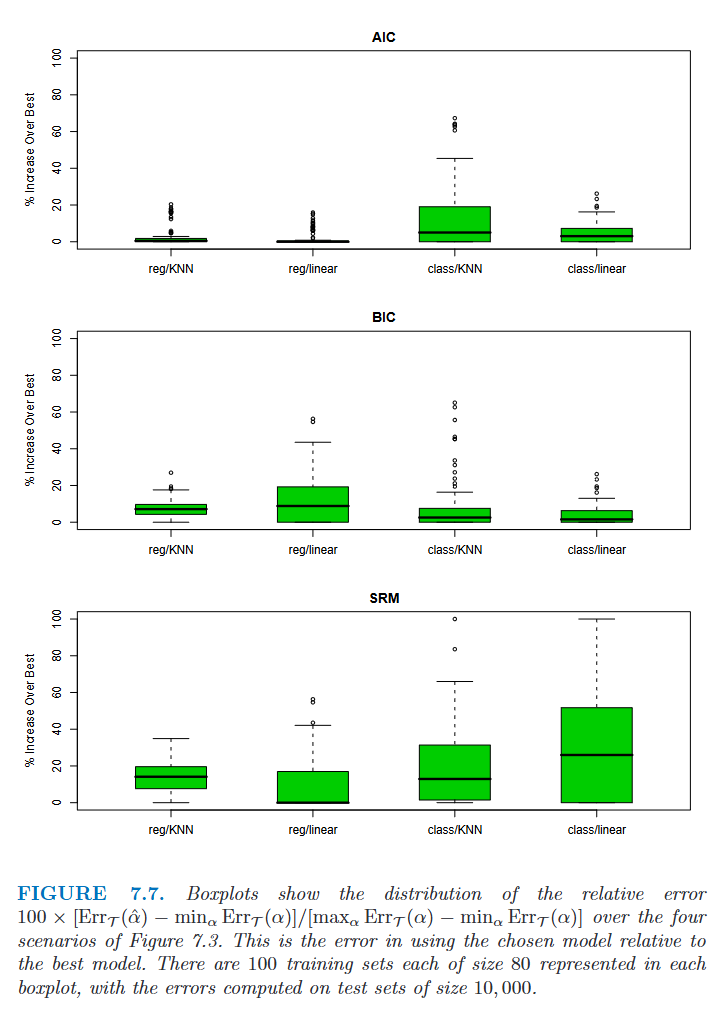
\includegraphics[width=0.95\textwidth]{Chapters/pic/ch_模型评估与选择/figure_7_7.png}
    \caption{箱线图展示图 7.3 四个场景下相对误差 $100 \times [\mathrm{Err}_{\mathcal{T}}(\hat{\alpha}) - \min_\alpha \mathrm{Err}_{\mathcal{T}}(\alpha)]/[\max_\alpha \mathrm{Err}_{\mathcal{T}}(\alpha) - \min_\alpha \mathrm{Err}_{\mathcal{T}}(\alpha)]$ 的分布——即使用所选模型相对于最佳模型的误差。每个箱线图代表 100 个大小为 80 的训练集，误差在大小为 10,000 的测试集上计算。}
    \label{fig:7_7}
\end{figure}

AIC 在所有四个场景中表现良好（即使 0-1 损失缺乏理论支持），BIC 表现接近，SRM 表现参差不齐。

% ============ §7.10 交叉验证 ============
\section{交叉验证}

交叉验证可能是估计预测误差最简单且最广泛使用的方法。该方法直接估计期望额外样本误差 $\mathrm{Err} = \E[L(Y, \hat{f}(X))]$——即将方法 $\hat{f}(X)$ 应用于来自 $X$ 和 $Y$ 联合分布的独立测试样本时的平均泛化误差。第 7.12 节将说明，交叉验证通常只能较好地估计期望预测误差，而非条件误差 $\mathrm{Err}_{\mathcal{T}}$。

\subsection{$K$ 折交叉验证}

将数据随机分为 $K$ 个大小大致相等的折。对第 $k$ 折，用其余 $K-1$ 折数据拟合模型，计算在第 $k$ 折上的预测误差。$K$ 折 CV 估计为：
\begin{equation}\label{eq:CV_K}
    \mathrm{CV}(\alpha) = \frac{1}{K}\sum_{k=1}^{K} \frac{1}{|F_k|}\sum_{i \in F_k} L(y_i, \hat{f}^{-k}_\alpha(x_i))
\end{equation}
其中 $\hat{f}^{-k}_\alpha$ 是剔除第 $k$ 折后拟合的模型，$F_k$ 为第 $k$ 折的索引集。

典型选择：$K = 5$ 或 $K = 10$。$K = N$ 的特例称为\textbf{留一交叉验证（LOOCV）}。

更精确地，设 $\kappa: \{1,\ldots,N\} \to \{1,\ldots,K\}$ 为指示观测 $i$ 分配到哪一折的索引函数，$\hat{f}^{-k}(x)$ 为剔除第 $k$ 折后拟合的函数。则 CV 预测误差估计为：
\begin{equation}\label{eq:CV}
    \mathrm{CV}(\hat{f}) = \frac{1}{N}\sum_{i=1}^{N} L\bigl(y_i, \hat{f}^{-\kappa(i)}(x_i)\bigr)
\end{equation}
对含调节参数 $\alpha$ 的模型族：
\begin{equation}\label{eq:CV_alpha}
    \mathrm{CV}(\hat{f}, \alpha) = \frac{1}{N}\sum_{i=1}^{N} L\bigl(y_i, \hat{f}^{-\kappa(i)}(x_i, \alpha)\bigr)
\end{equation}
选择使 $\mathrm{CV}(\hat{f}, \alpha)$ 最小的 $\hat{\alpha}$，再用全部数据拟合最终模型 $f(x, \hat{\alpha})$。

这里容易混淆：LOOCV（$K=N$）并非一种不同的做法——它仍是 $K$ 折 CV，只是每折恰好包含 1 个观测。以 $N=100$ 为例，5 折 CV 每次用 80 个训练、20 个验证，共做 5 次；LOOCV 每次用 99 个训练、1 个验证，共做 100 次。LOOCV 的每个训练集几乎等于全量数据（只差一个点），因此偏差极低；但 100 个训练集高度相似，导致方差大。

\textbf{最终模型用什么训练？} CV 全程只用原始训练集——从未见过独立的测试集。CV 的作用仅仅是选 $\hat{\alpha}$。选定后，用\textbf{全部 $N$ 个观测}重新训练一次，得到最终模型 $\hat{f}(\cdot, \hat{\alpha})$。测试集（如果保留了一份）只在最后评估这个最终模型时使用一次。

\textbf{一个具体流程示例。} 假设有 $N=150$ 条数据，要做岭回归，调节参数 $\alpha$ 候选为 $\{0.01, 0.1, 1, 10, 100\}$。

\begin{enumerate}
    \item 随机打乱数据，分成 5 折（每折 30 条）。
    \item 对每个候选 $\alpha$：
    \begin{itemize}
        \item 第 1 折做验证，第 2--5 折（120 条）训练 → 算验证误差 $e_1(\alpha)$
        \item 第 2 折做验证，其余训练 → $e_2(\alpha)$
        \item $\cdots$ 共 5 次，取平均 $\mathrm{CV}(\alpha) = \frac{1}{5}\sum_{k=1}^{5} e_k(\alpha)$
    \end{itemize}
    \item 选 $\hat{\alpha} = \argmin_\alpha \mathrm{CV}(\alpha)$，假设结果为 $\hat{\alpha}=1$。
    \item \textbf{用全部 150 条数据}，以 $\alpha=1$ 做岭回归 → 得到最终模型 $\hat{\beta}^{\text{ridge}}_{\alpha=1}$。
    \item （可选）在保留的独立测试集上评估该模型的泛化误差。
\end{enumerate}

整个过程没有用到测试集来选 $\alpha$——这正是 CV 的核心价值：在训练数据内部模拟「训-验」分离。

\subsection{$K$ 的选择：偏差-方差权衡}

CV 实际估计的是什么？$K=5$ 或 $10$ 时，每折的训练集与原训练集差别较大，估计的应是 $\mathrm{Err}$（期望误差）。$K=N$（LOOCV）时，训练集几乎与原集相同，可能更接近 $\mathrm{Err}_{\mathcal{T}}$。但第 7.12 节将说明，CV 通常只能有效估计 $\mathrm{Err}$。

\begin{itemize}
    \item \textbf{$K=N$（LOOCV）：} 近似无偏（对 $\mathrm{Err}$），但方差高——$N$ 个训练集高度相似。
    \item \textbf{$K=5$ 或 $10$：} 方差低，但若学习曲线在给定训练集大小处有显著斜率，则会有偏差。
\end{itemize}

\begin{figure}[htbp]
    \centering
    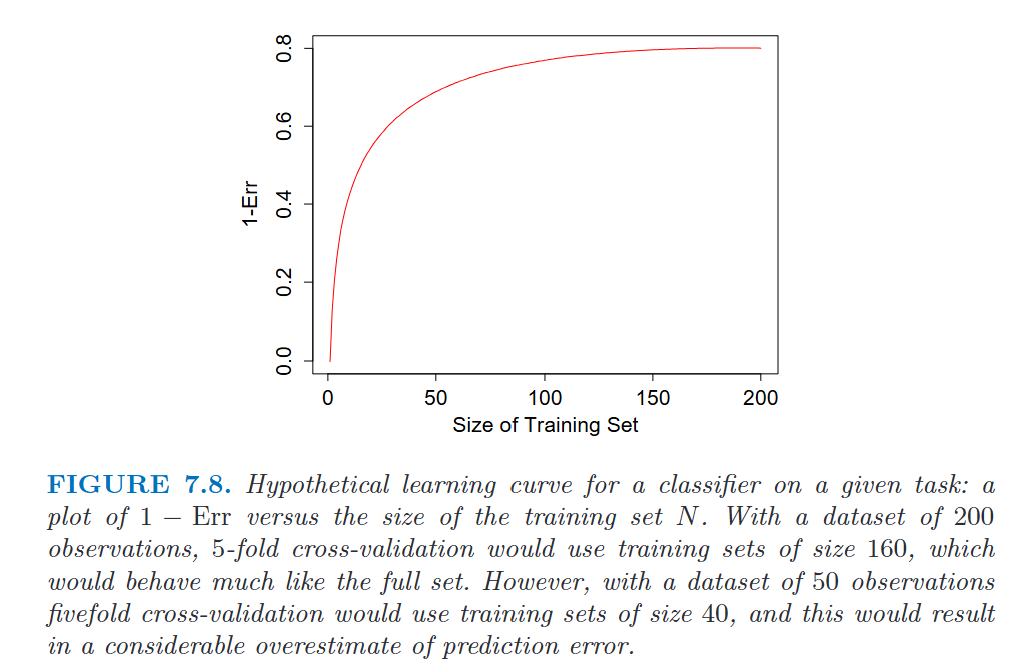
\includegraphics[width=0.7\textwidth]{Chapters/pic/ch_模型评估与选择/figure_7_8.png}
    \caption{某个分类任务假设的学习曲线：$1-\mathrm{Err}$ 随训练集大小 $N$ 的变化。若数据集有 200 个观测，5 折 CV 使用大小为 160 的训练集，其表现与全量集几乎相同。但若仅有 50 个观测，5 折 CV 使用大小为 40 的训练集，将导致显著高估预测误差。}
    \label{fig:7_8}
\end{figure}

总体建议：5 折或 10 折 CV 作为折中方案。

\subsection{广义交叉验证（GCV）}

GCV 为线性拟合方法在平方误差损失下的 LOOCV 提供方便的近似。对线性拟合 $\hat{\mathbf{y}} = \mathbf{S}\mathbf{y}$：
\begin{equation}\label{eq:GCV}
    \mathrm{GCV}(\hat{f}) = \frac{1}{N}\sum_{i=1}^{N} \left[\frac{y_i - \hat{f}(x_i)}{1 - \trace(\mathbf{S})/N}\right]^2
\end{equation}
其中 $\trace(\mathbf{S})$ 是有效参数个数。当 $\trace(\mathbf{S})$ 比单个 $S_{ii}$ 更易计算时，GCV 有计算优势。在光滑问题中，GCV 还可缓解 CV 的欠光滑倾向。

GCV 与 AIC 的联系：利用近似 $1/(1-x)^2 \approx 1+2x$ 可见其相似性。

\subsection{交叉验证的正确与错误做法}

\textbf{常见错误：} 先在全量数据上做变量筛选（如选与标签最相关的 100 个预测变量），再对筛选后的数据做 CV。这相当于筛选出的变量「已经见过」被留出的样本——CV 误差会严重偏低。

\textbf{仿真示例：} $N=50$，$p=5000$ 个与标签独立的预测变量，真实误差率 50\%。先用全量数据选 100 个最相关变量，再对 1-NN 做 CV → 平均 CV 误差仅 3\%（严重错误）。

\begin{figure}[htbp]
    \centering
    \begin{tikzpicture}[
        node distance=0.8cm and 1.2cm,
        box/.style={draw, rounded corners, fill=gray!8, text width=2.6cm, align=center, minimum height=0.8cm, font=\small},
        badbox/.style={draw, rounded corners, fill=red!8, text width=2.6cm, align=center, minimum height=0.8cm, font=\small},
        goodbox/.style={draw, rounded corners, fill=green!8, text width=2.6cm, align=center, minimum height=0.8cm, font=\small},
        arrow/.style={->, >=stealth, thick},
        badarrow/.style={->, >=stealth, thick, red!70},
        goodarrow/.style={->, >=stealth, thick, green!50!black}
    ]

    % === 错误做法 ===
    \node[badbox, text width=5cm, minimum height=0.6cm, font=\small\bfseries] (badtitle) at (0, 0) {✗ 错误做法：先筛选，再 CV};

    \node[badbox, below=0.4cm of badtitle] (bad1) {全量数据\\($N$ 条)};
    \node[badbox, right=of bad1] (bad2) {变量筛选\\(选相关性最高的)};
    \node[badbox, right=of bad2] (bad3) {划分折};
    \node[badbox, below=of bad3] (bad4) {逐折 CV};
    \node[badbox, left=of bad4, text width=3.5cm] (bad5) {CV 误差 $\approx 3\%$\\真实误差 $=50\%$};

    \draw[badarrow] (bad1) -- (bad2);
    \draw[badarrow] (bad2) -- (bad3);
    \draw[badarrow] (bad3) -- (bad4);
    \draw[badarrow] (bad4) -- (bad5);

    \node[font=\footnotesize\itshape, text=red!70, below=0.2cm of bad5, text width=4.5cm, align=center] {筛选时「偷看」了被留出样本的标签};

    % === 正确做法 ===
    \node[goodbox, text width=5cm, minimum height=0.6cm, font=\small\bfseries] (goodtitle) at (0, -5.5) {✓ 正确做法：CV 包裹整个流程};

    \node[goodbox, below=0.4cm of goodtitle] (good1) {全量数据\\($N$ 条)};
    \node[goodbox, right=of good1] (good2) {划分 $K$ 折};
    \node[goodbox, right=of good2, text width=3.8cm] (good3) {对每折 $k=1,\ldots,K$：};
    \node[goodbox, below=of good3] (good4) {筛选变量\\(仅用训练折)};
    \node[goodbox, left=of good4] (good5) {训练模型\\(仅用训练折)};
    \node[goodbox, left=of good5] (good6) {验证折 $k$ 上评估};
    \node[goodbox, below=of good6, text width=3.5cm] (good7) {CV 误差 $\approx 50\%$\\真实误差 $=50\%$};

    \draw[goodarrow] (good1) -- (good2);
    \draw[goodarrow] (good2) -- (good3);
    \draw[goodarrow] (good3) -- (good4);
    \draw[goodarrow] (good4) -- (good5);
    \draw[goodarrow] (good5) -- (good6);
    \draw[goodarrow] (good6) -- (good7);

    \node[font=\footnotesize\itshape, text=green!50!black, below=0.2cm of good7, text width=4.5cm, align=center] {每折独立筛选，不会泄露验证折信息};

    \end{tikzpicture}
    \caption{交叉验证的错误做法与正确做法对比。上图：先在全量数据上做变量筛选再划分折——筛选时已「偷看」了所有样本的标签，导致 CV 误差严重偏低。下图：先划分折，在每折的训练部分独立筛选变量和训练——CV 误差无偏。}
    \label{fig:cv_wrong_right}
\end{figure}

\begin{figure}[htbp]
    \centering
    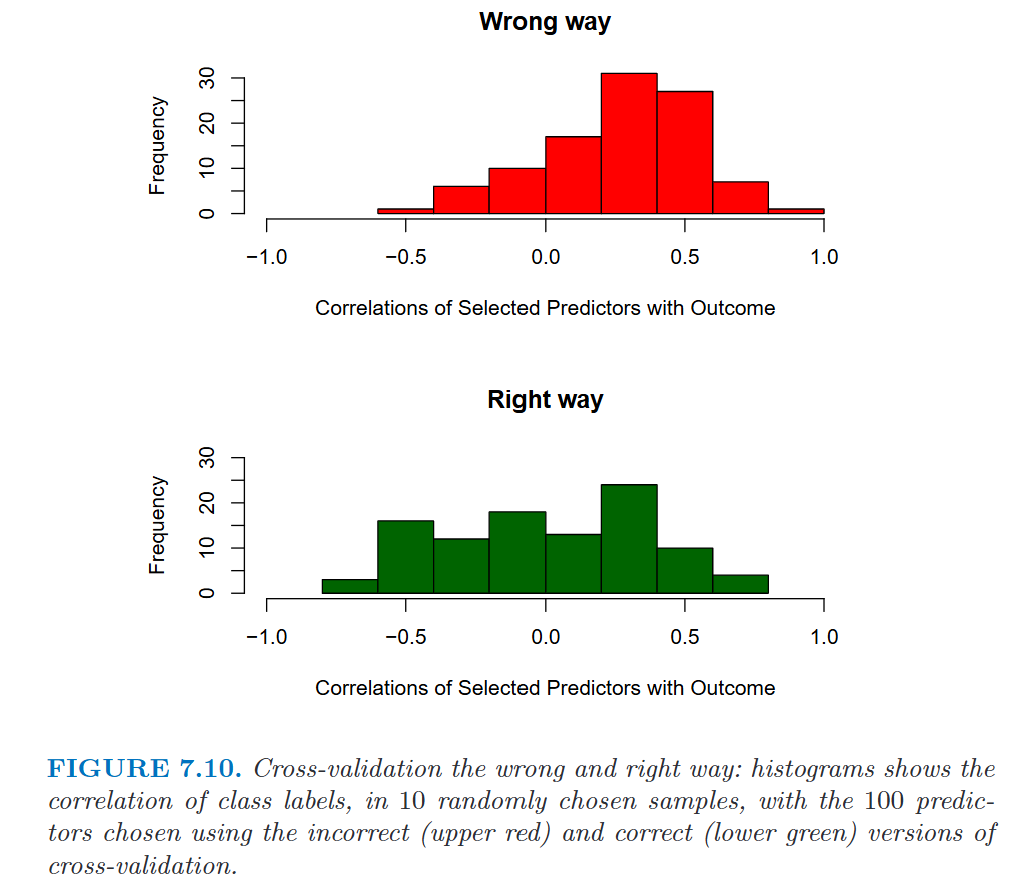
\includegraphics[width=0.8\textwidth]{Chapters/pic/ch_模型评估与选择/figure_7_10.png}
    \caption{交叉验证的错误与正确方式：直方图展示了在 10 个随机选择的样本中，使用错误（上，红色）和正确（下，绿色）CV 方式所选 100 个预测变量与类别标签的相关性。错误方式下相关性被人为夸大。}
    \label{fig:7_10}
\end{figure}

这里「变量筛选」指的是\textbf{从众多预测变量中挑选出一个子集}——选列，而非选值。例如从 5000 个基因中挑出与标签 $Y$ 最相关的前 100 个，扔掉其余 4900 个：
$$
X_1, X_2, \ldots, X_{5000} \;\xrightarrow{\text{按相关性排序截断}}\; X_{(1)}, X_{(2)}, \ldots, X_{(100)}
$$
筛选方法：对每个变量 $j$ 单独计算 $|r_j| = |\mathrm{Cor}(X_j, Y)|$，排序取最大的若干个。每折独立做——用该折的 40 个训练样本算相关性、独立排序、独立截断，各折选出的变量\textbf{通常不同}，不取平均。

\textbf{完整流程演示（$N=50$，$p=5000$，5 折 CV，1-NN 分类器）：}

\begin{enumerate}
    \item 随机将 50 人分成 5 折，每折 10 人。
    \item \textbf{第 1 折做验证：} 用折 2--5 的 40 人，对 5000 个基因逐一算 $|r_j|$，取前 100 个。用这 100 个基因和 40 人训练 1-NN，在折 1 的 10 人上算误差 $e_1$。
    \item \textbf{第 2 折做验证：} 用折 1,3,4,5 的 40 人，\textbf{重新}算 $|r_j|$、\textbf{重新}选前 100（可能与折 1 不同！），训练并算 $e_2$。
    \item 第 3--5 折同理，分别得 $e_3, e_4, e_5$。
    \item $\mathrm{CV} = \frac{1}{5}(e_1 + \cdots + e_5)$。CV 的作用至此完成——它给出了用 100 个基因时 1-NN 的期望误差估计。
    \item \textbf{训练最终模型：} 回到全量 50 人，重新算 $|r_j|$（这次用全部 50 人），取前 100 个基因。用这 100 个基因和全部 50 人训练最终 1-NN 分类器。这 100 个基因可能与任一折选出的都不同——这是正常的，因为现在是用全量数据筛选。
    \item \textbf{最终评估：} 在独立的测试集（从未参与上述任何步骤）上评估最终模型的泛化误差。
\end{enumerate}

错误做法的区别仅在于第 1 步之前：先用全部 50 人算 $|r_j|$、一次性选出 100 个基因，此后各折\textbf{不再重新筛选}——这 100 个基因在筛选时已「见过」全部 50 人的标签，导致 CV 误差虚低。

这里有一个容易困惑的点：既然 CV 时每折独立筛选、最终训练又回到全量数据重新筛选，那 CV 到底做了什么决策？CV 的目的不是训练最终模型，而是\textbf{评估和选择方案}。比如你同时考虑三种方案——用 50 个基因、100 个基因、200 个基因——CV 分别给出它们的泛化误差估计，你据此选择最合适的方案（如 100 个基因）。决策完成后 CV 使命结束。最后一步用全量数据重新筛选 100 个基因并训练，是\textbf{充分利用所有数据产出最佳模型}——此时不再需要验证，用全量数据筛选不违反任何原则。两个阶段的分工：CV 负责选超参数，最终训练负责出模型。

\textbf{正确做法：} CV 必须应用于\textbf{整个建模流程}——样本必须在任何筛选步骤之前被留出。对 $K$ 折 CV 的第 $k$ 折：
\begin{enumerate}
    \item 用除第 $k$ 折外的样本筛选「好」变量
    \item 用除第 $k$ 折外的样本构建分类器
    \item 在第 $k$ 折上评估
\end{enumerate}
唯一的例外是\textbf{无监督}的初始筛选（如按方差选变量）可在留出样本前进行——因为它不涉及标签，不会给变量不公平的优势。

\subsection{交叉验证真的有效吗？——高维示例}

考虑 $N=20$（两类各半），$p=500$ 个与标签独立的标准高斯预测变量，真实误差率 50\%。使用单变量树桩（stump）分类器。简单论证认为 CV 会失败：因为全量数据上总能找到一个分裂得很好的预测变量，它在任何 4/5 和 1/5 子集上也应分裂得好。

图 7.11 的仿真表明这个论证是\textbf{错误}的——关键在于\textbf{分割点必须在 CV 的每折中重新估计}。对 50 个模拟数据集的 5 折 CV，平均误差率约为 50\%，正是真实的期望预测误差。不过 CV 估计的变异性很大，报告 CV 估计的标准误差很重要。

% ============ §7.11 自助法 ============
\section{自助法（Bootstrap）}

自助法是一种评估统计准确性的通用工具。与交叉验证类似，Bootstrap 试图估计条件误差 $\mathrm{Err}_{\mathcal{T}}$，但通常只能较好地估计期望预测误差 $\mathrm{Err}$。

\subsection{基本思想}

设训练集为 $\mathbf{Z} = (z_1, z_2, \ldots, z_N)$，其中 $z_i = (x_i, y_i)$。基本做法是从 $\mathbf{Z}$ 中有放回地随机抽取 $N$ 个样本，形成一个 Bootstrap 样本 $\mathbf{Z}^{*b}$。重复 $B$ 次（如 $B=100$），对每个 $\mathbf{Z}^{*b}$ 拟合模型 $\hat{f}^{*b}(x)$。

\subsection{Bootstrap 估计预测误差}

一种自然的做法是用 Bootstrap 样本上的表现来估计误差。但直接使用会出现问题——Bootstrap 样本与原始训练集有重叠。常用方法包括：
\begin{itemize}
    \item \textbf{留一 Bootstrap：} 对观测 $i$，仅使用不含 $i$ 的 Bootstrap 样本来预测 $i$。
    \item \textbf{$.632$ 估计：} 结合训练误差和留一 Bootstrap 误差的加权平均。
\end{itemize}

更详细的内容见第 7.11 节后续。
